\documentclass[12pt]{article}
\usepackage{geometry} % Pour passer au format A4
\geometry{hmargin=1cm, vmargin=1cm} % 

% Page et encodage
\usepackage[T1]{fontenc} % Use 8-bit encoding that has 256 glyphs
\usepackage[english,french]{babel} % Français et anglais
\usepackage[utf8]{inputenc} 

\usepackage{lmodern}
\setlength\parindent{0pt}

% Graphiques
\usepackage{graphicx,float,grffile}

% Maths et divers
\usepackage{amsmath,amsfonts,amssymb,amsthm,verbatim}
\usepackage{multicol,enumitem,url,eurosym,gensymb}

% Sections
\usepackage{sectsty} % Allows customizing section commands
\allsectionsfont{\centering \normalfont\scshape}

% Tête et pied de page

\usepackage{fancyhdr} 
\pagestyle{fancyplain} 

\fancyhead{} % No page header
\fancyfoot{}

\renewcommand{\headrulewidth}{0pt} % Remove header underlines
\renewcommand{\footrulewidth}{0pt} % Remove footer underlines

\newcommand{\horrule}[1]{\rule{\linewidth}{#1}} % Create horizontal rule command with 1 argument of height

%----------------------------------------------------------------------------------------
%   Début du document
%----------------------------------------------------------------------------------------

\begin{document}

%----------------------------------------------------------------------------------------
% RE-DEFINITION
%----------------------------------------------------------------------------------------
% MATHS
%-----------

\newtheorem{Definition}{Définition}
\newtheorem{Theorem}{Théorème}
\newtheorem{Proposition}{Propriété}

% MATHS
%-----------
\renewcommand{\labelitemi}{$\bullet$}
\renewcommand{\labelitemii}{$\circ$}
%----------------------------------------------------------------------------------------
%   Titre
%----------------------------------------------------------------------------------------

\setlength{\columnseprule}{1pt}

\horrule{2px}
\section*{Chapitre 4 - Théorème de Pythagore}
\horrule{2px}

\section*{1 - Deux outils mathémmatiques}

On appelle des outils mathématiques des fonctions. Elles ont un sens géométrique et un sens numérique. Pour réussir le chapitre de Pythagore, il faut comprendre ces deux aspects. 

\begin{multicols}{2}

\subsection*{La fonction carré}

  \begin{figure}[H]
        \centering
        \includegraphics[width=0.8\linewidth]{4x4-pythagore/sources/fonction-carre.pdf}
  \end{figure}

\begin{itemize}
\item Elle est noté $x^2$. 
\item La fonction carré permet de calculer l'aire d'un carré à partir de son côté.
\item $15^2 = 15 \times 15 = 225$
\end{itemize}
\underline{Liste des premiers carrés :}

	\begin{itemize}
		\item $1^2 = 1 \times 1 = 1$
		\item $2^2 = 2 \times 2 = 4$
		\item $3^2 = 3 \times 3 = 9$
		\item $4^2 = 4 \times 4 = 16$
		\item $5^2 = 5 \times 5 = 25$
		\item $6^2 = 6 \times 6 = 36$
		\item $7^2 = 7 \times 7 = 49$
		\item $8^2 = 8 \times 8 = 64$
		\item $9^2 = 9 \times 9 = 81$
		\item $10^2 = 10 \times 10 = 100$
		\item $11^2 = 11 \times 11 = 121$
		\item $12^2 = 12 \times 12 = 144$
	\end{itemize}

\subsection*{La fonction racine carré}

  \begin{figure}[H]
        \centering
        \includegraphics[width=0.8\linewidth]{4x4-pythagore/sources/fonction-racine.pdf}
  \end{figure}

\begin{itemize}
\item Elle est noté $\sqrt{x}$. 
\item La fonction racine carré permet de calculer le côté d'un carré à partir de son aire.
\item C'est une nouvelle opération qui ne peut être écrit avec les 4 opérations de base. Par définition : $\sqrt{12}^2 = 12$.
\end{itemize}
	\underline{Liste des premières racines : }

	\begin{itemize}
		\item $\sqrt{1} = 1$
		\item $\sqrt{4} = 2$
		\item $\sqrt{9} = 3$
		\item $\sqrt{16} = 4$
		\item $\sqrt{25} = 5$
		\item $\sqrt{36} = 6$
		\item $\sqrt{49} = 7$
		\item $\sqrt{64} = 8$
		\item $\sqrt{81} = 9$
		\item $\sqrt{100} = 10$
		\item $\sqrt{121} = 11$
		\item $\sqrt{144} = 12$
	\end{itemize}

\end{multicols}

\newpage

\section*{2 - Théorème géométrique}

Dans un triangle rectangle, la somme des deux petits carrés est égale au grand carré.

\paragraph{source} : \url{youtu.be}

  \begin{figure}[H]
        \centering
        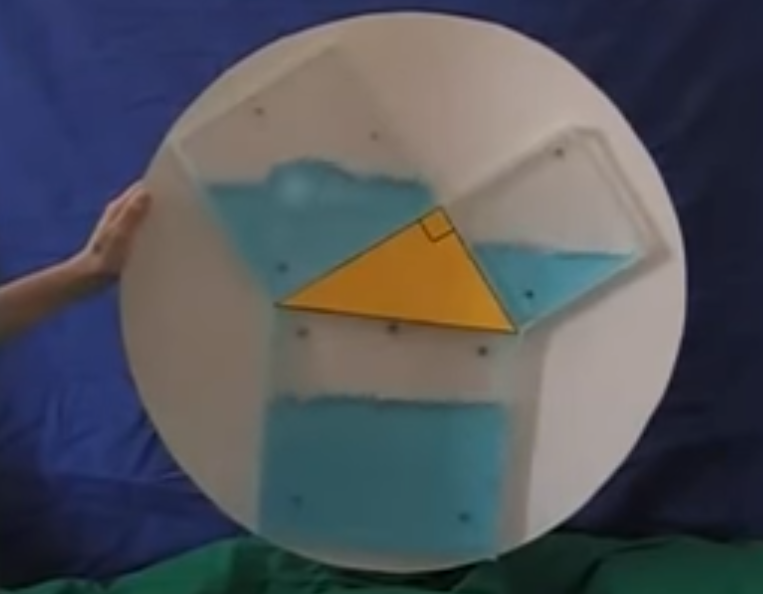
\includegraphics[width=0.6\linewidth]{4x4-pythagore/sources/pyth.png}
  \end{figure}

\section*{3 - Modélisation : Usage du théorème}

\subsection*{3.1 - Calcul de Longueur}

Si dans un triangle rectangle, je connais deux longueurs, je vais pouvoir calculer la troisième longueur.

\begin{multicols}{2}

	\subsubsection*{a. Recherche du grand côté : (+)}

	\begin{figure}[H]
		\centering
		\includegraphics[width=0.5\linewidth]{4x4-pythagore/sources/re-h.pdf}
	\end{figure}

	Dans le triangle MNO rectangle en O.\\
	D'après le théorème de Pythagore.
	\begin{eqnarray*}
		MN^2 &=& MO^2 + NO^2 \\
		MN^2 &=& 20^2 + 32^2 \\
		MN   &=& \sqrt{20^2 + 32^2} \\
		MN   &\approx& 37.7
	\end{eqnarray*}

	La longueur MN mesure environ 27.7cm.


\end{multicols}
\begin{multicols}{2}
	\subsubsection*{b. Recherche d'un petit côté (-)}

	\begin{figure}[H]
		\centering
		\includegraphics[width=0.5\linewidth]{4x4-pythagore/sources/re-c.pdf}
	\end{figure}

	Dans le triangle MNO rectangle en O.\\
	D'après le théorème de Pythagore.
	\begin{eqnarray*}
		MN^2 &=& MO^2 + NO^2 \\
		40^2 &=& MO^2 + 12^2 \\
		MO   &=& \sqrt{40^2 - 12^2} \\
		MO   &=& 38
	\end{eqnarray*}

	La longueur MO mesure 38cm.

\end{multicols}

\newpage

\subsubsection*{c. Problème}

\textbf{Énoncé} J'ai oublié mes clés pour rentrer chez moi. La fenêtre du premier étage est ouverte.
Le bas de la fenêtre se trouve à 4m du sol. Un voisin me prête une échelle de 4.5m de long.
Pour monter à l'échelle sans tomber, je suis obligé de poser les pieds de l'échelle à 1.5 m du pied du mur.\\
\textbf{Pourrai-je atteindre le bas de ma fenêtre ?}

\begin{multicols}{2}

	\textbf{Je représente la situation}

	\begin{figure}[H]
		\centering
		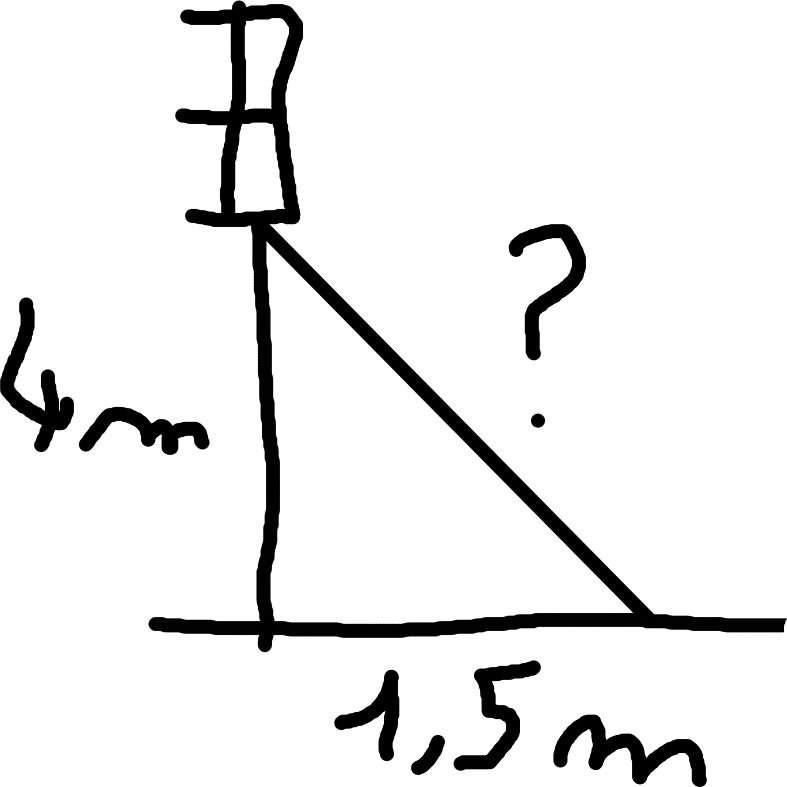
\includegraphics[width=0.5\linewidth]{4x4-pythagore/sources/probleme.jpg}
	\end{figure}

	\textit{J'ai un triangle rectangle, j'ai deux longueurs, je cherche la troisième pour la comparer avec l'échelle.}\\
	\textbf{Je peux utiliser le théorème de Pythagore.}
	\vspace{1cm}
	\paragraph{Rédiger}
  On appelle $x$ la longueur cherchée.\\
	Le triangle est rectangle.\\
	D'après le théorème de Pythagore.

	\begin{eqnarray*}
		x^2 &=& 4^2 + 1.5^2 \\
		x   &=& \sqrt{4^2 + 1.5^2} \\
		x   &\approx& 4.27
	\end{eqnarray*}

	Comme 4.27m < 4.5m, \textit{(la longueur x entre la fenêtre et le sol est plus petite que l'échelle.)}\\
	\textbf{L'echelle est suffisament grande.}
\end{multicols}

\subsection*{3.2 Démonstration}

Si on connaît les trois côtés d'un triangle, on peut démontrer si le triangle est rectangle. Pour cela on compare le grand carré avec la somme des autres carrés.

\begin{multicols}{2}
Soit DMW un triangle tel que : DW = 14,8 cm , WM = 4,8 cm et DM = 14 cm.\\
Quelle est la nature du triangle DMW ?\\

Le triangle DMW n’est ni isocèle, ni équilatéral.\\
$DW^2 = 14,8^2 = 219,04$ ($[DW]$ est le plus grand côté.) \\
$WM^2 + DM^2 = 4,8^2 + 14^2 = 219,04$\\
Donc $DW^2 = WM^2 + DM^2$.\\

D’après la réciproque du théorème de Pythagore, le triangle $DMW$ est rectangle en $M$.\\


Soit ZHB un triangle tel que : HZ = 19,3 cm, HB = 20 cm et BZ = 5,6 cm.\\
Quelle est la nature du triangle ZHB ?\\

Le triangle ZHB n’est ni isocèle, ni équilatéral.\\
$HB^2 = 20^2 = 400$  ($[HB]$ est le plus grand côté.)\\
$BZ^2 + HZ^2 = 5,6^2 + 19,3^2 = 403,85$\\
Donc $HB^2 \neq BZ^2 + HZ^2$.\\

D’après la contraposée du théorème de Pythagore, le triangle $ZHB$ n'est rectangle.\\
\end{multicols}

\end{document}
